\section{Auxiliary circle of an ellipse and the affine transformation view}

Let $\ell$ be the major axis and let $O$ be the center of the ellipse. Recall that the ellipse has semi-major axis $a$ and semi-minor axis $b$. Consider the \emph{major-axis circle} $\mathcal C$: the circle centered at $O$ with radius $a$ (so its diameter equals the major axis length $2a$). This is also the standard \emph{auxiliary circle} associated to the ellipse.

Define the affine map $\Phi$ geometrically as follows. For any point $P$ in the plane, let $P_T$ be the foot of the perpendicular from $P$ to $\ell$. On the same perpendicular line $P_TP$ choose a point $P_0$ on the same side of $\ell$ as $P$ such that
\begin{equation}
  P_TP_0=\frac{b}{a}\,P_TP.
\end{equation}
Then set $\Phi(P):=P_0$.

Equivalently, $\Phi$ fixes $\ell$ pointwise and scales all lengths perpendicular to $\ell$ by the constant factor $b/a$. This map sends lines to lines, preserves parallelism, and scales all areas by $b/a$. In the standard auxiliary circle construction, $\Phi$ maps $\mathcal C$ to the ellipse.

\paragraph{Tangents via secants (Newton's 1687 viewpoint).}
Newton often treats a tangent as the \emph{ultimate position} of a secant: if $A$ is a point on the curve and $B$ is a nearby point, then the chord line $AB$ approaches the tangent line at $A$ as $B\to A$ (in Newton's 1687 language, as one takes the ``ultimate ratio''). In our setting this provides an alternative justification for the fact that $\Phi$ carries circle tangents to ellipse tangents.

Indeed, let $A_0\in\mathcal C$ correspond to $A=\Phi(A_0)$ on the ellipse, and let $B_0\in\mathcal C$ correspond to $B=\Phi(B_0)$. Since $\Phi$ is affine, it maps the secant (chord) line $A_0B_0$ to the secant line $AB$, and it preserves incidences and parallelism. As $B_0\to A_0$, the secant line $A_0B_0$ approaches the tangent to $\mathcal C$ at $A_0$, while $AB$ approaches the tangent to the ellipse at $A$. Therefore, in the same limiting (secant-to-tangent) sense, $\Phi$ maps the circle tangent at $A_0$ to the ellipse tangent at $A$.

\begin{figure}[t]
  \centering
  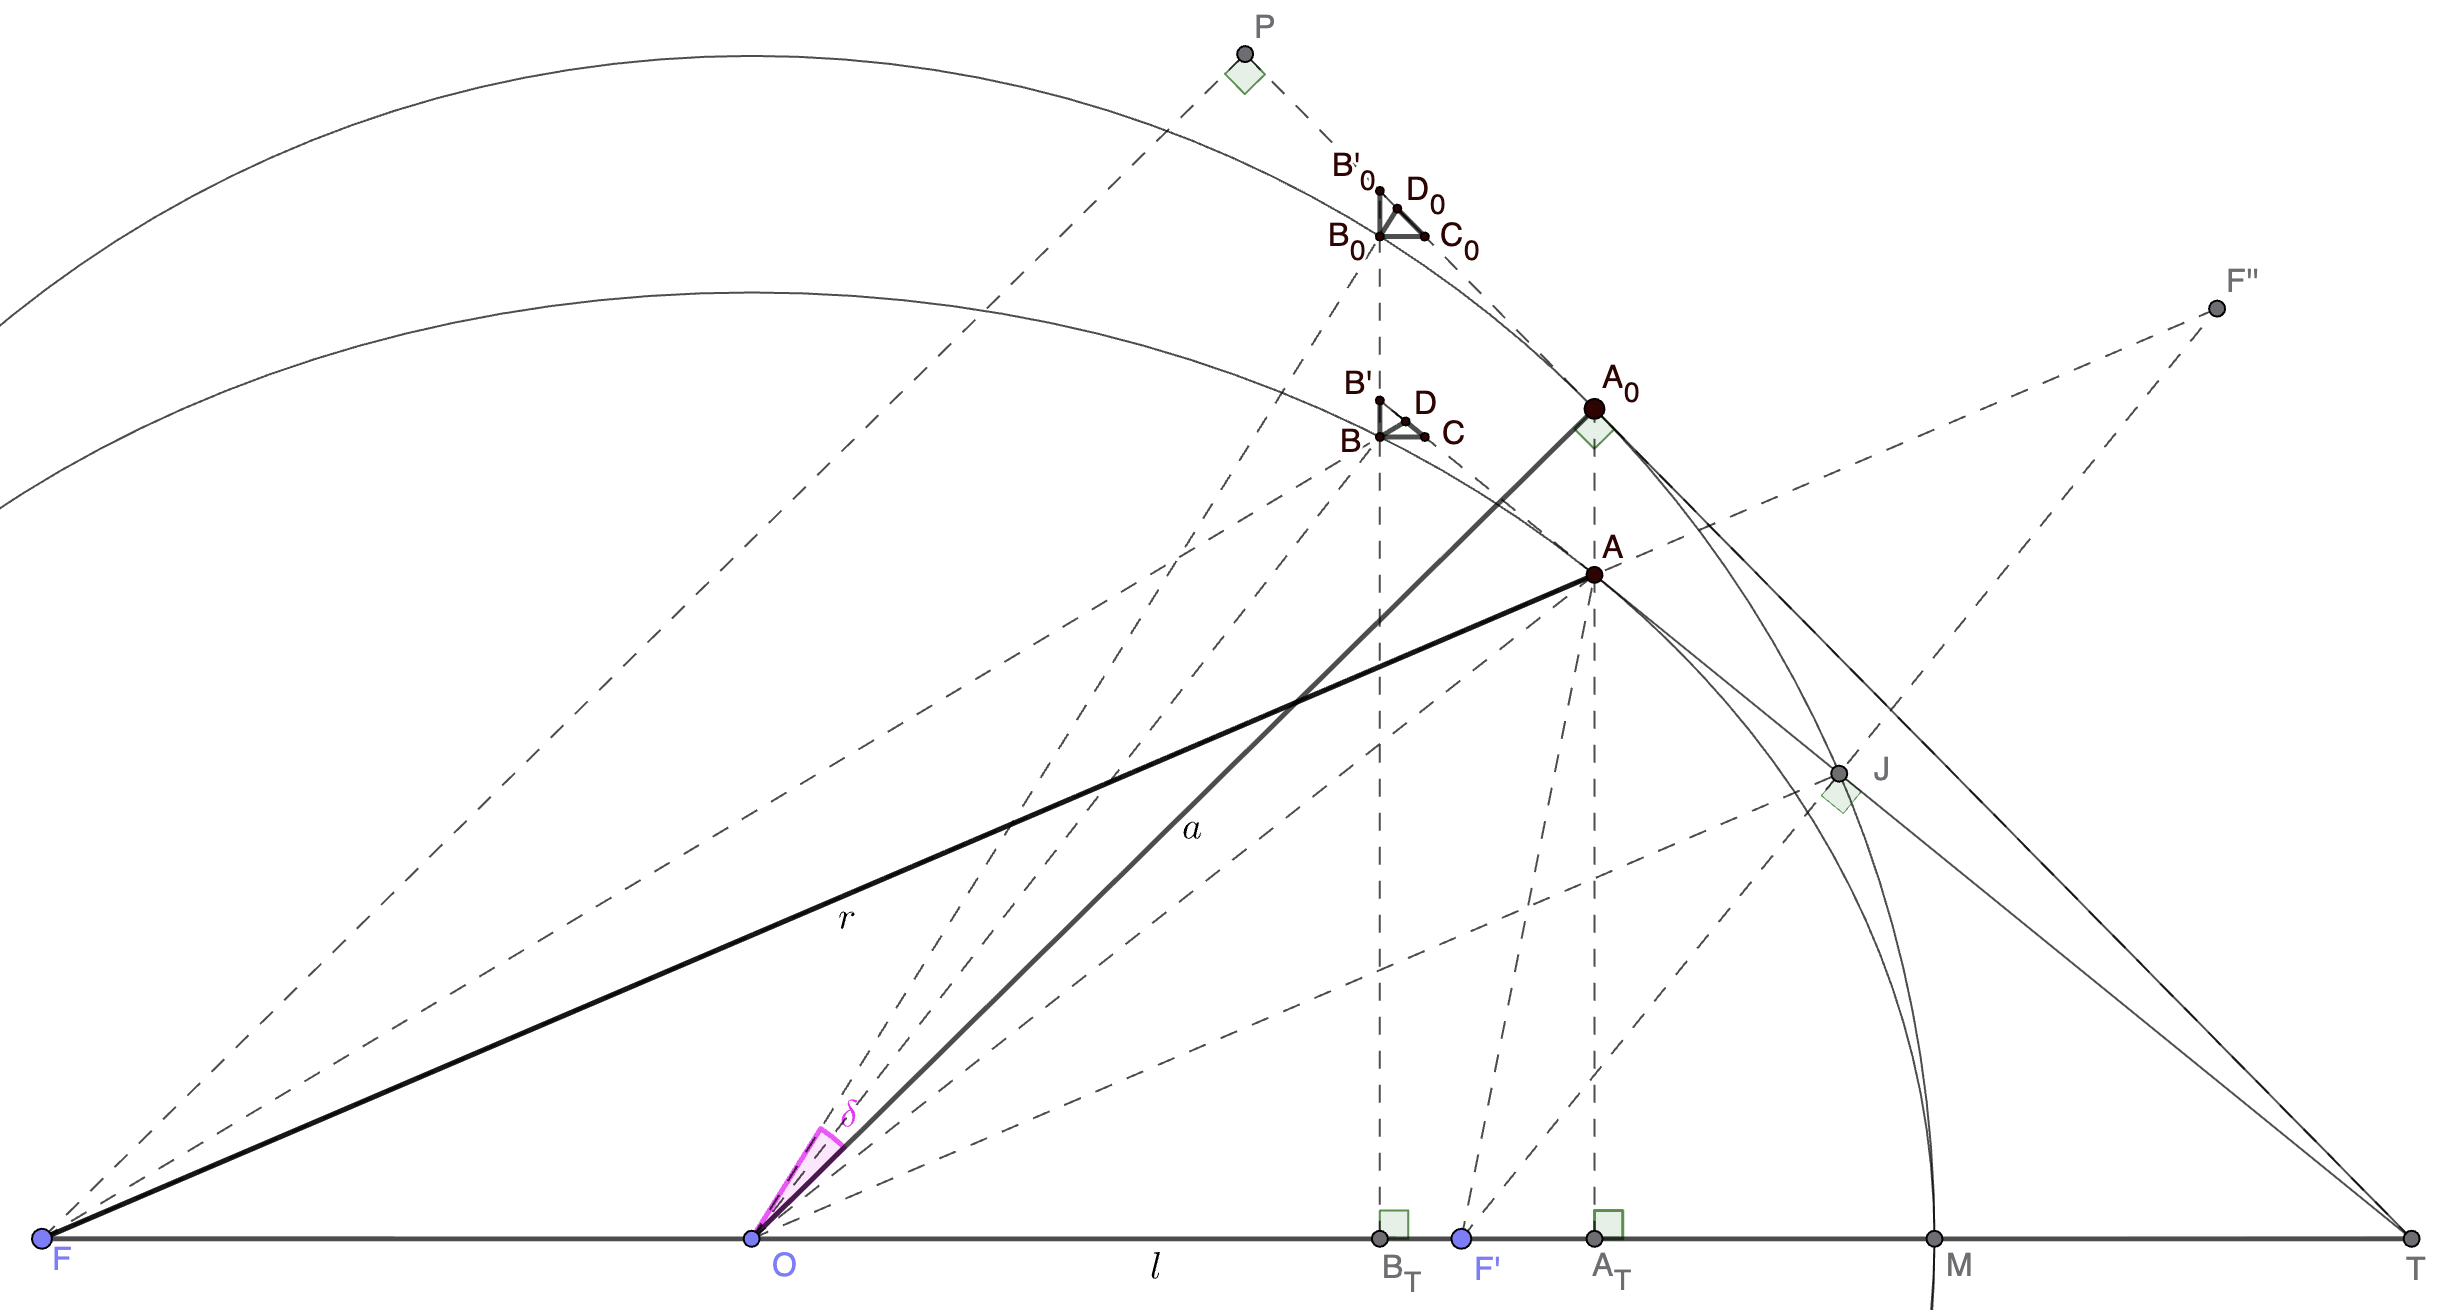
\includegraphics[width=\linewidth]{assets/images/MotionFigure.png}
  \caption{Affine relation of motion between the auxiliary circle and the ellipse.}
  \label{fig:affine-relation-of-motion}
\end{figure}

A few simple geometric consequences we use repeatedly in this section:
\begin{itemize}
  \item Straight lines map to straight lines under $\Phi$.
  \item Horizontal lengths (parallel to $\ell$) are unchanged by $\Phi$.
  \item Vertical lengths (perpendicular to $\ell$) scale by $b/a$.
  \item Parallel lines stay parallel under $\Phi$, and ratios of lengths along such lines are unchanged by $\Phi$.
  \item Areas scale by $b/a$.
  \item The inverse map $\Phi^{-1}$ sends $\Phi(A)$ back to $A$ and scales vertical lengths by $a/b$.
\end{itemize}
Although Newton (1687) did not formulate affine transformations explicitly, he repeatedly used equivalent geometric invariance principles. For example, Markowsky's reconstruction of Proposition~6 shows that, for an ellipse, the product of the ordinate to a conjugate diameter and the semi-length of that conjugate diameter is constant; this is an affine invariant arising from the circle-to-ellipse map \cite{markowsky2011newton}. Newton uses this same type of fact in Proposition~XI \cite{newton1846mottewikisource}. Likewise, in Book~I, Proposition~XXXI (Problem~XXIII) and its Scholium, Newton's computation of time along a given ellipse relies on area scaling between the auxiliary circle and the ellipse \cite{newton1846mottewikisource,chandrasekhar1995principia}.

\subsection{Tangent transfer and matching normal drops}

In the remainder of this section, we use \Cref{fig:affine-relation-of-motion} as the setup for understanding motion on the ellipse through its auxiliary circle. We now record a concrete straightedge-and-compass configuration that makes the affine ``transport'' of the short-time normal departure from the tangent explicit.
The purpose of this section is to obtain the geometric local-drop estimate; the kinematic conversion to acceleration then uses \Cref{lem:deflection-identity,lem:bd-over-br2} from Section~2.

\subsubsection{Circle companions and tangent transfer}

Let $\ell$ be the major axis, and let $\Phi$ map the auxiliary circle $\mathcal{C}$ to the ellipse. From $A$ and $B$ drop perpendiculars to $\ell$ and extend these same vertical lines to meet the auxiliary circle $\mathcal C$ at $A_0$ and $B_0$ (choose the intersections on the same side of $\ell$ as $A$ and $B$). By construction, $\Phi(A_0)=A$ and $\Phi(B_0)=B$.
Draw the tangent to $\mathcal C$ at $A_0$ and let it meet $\ell$ at $T$.

\begin{lemma}[Tangent transfer with fixed $T$]
  \label[lemma]{lem:tangent-transfer}
  Under $\Phi$, the circle tangent at $A_0$ maps to the ellipse tangent at $A$. Moreover, since $\Phi$ fixes $\ell$ pointwise, the intersection point $T\in\ell$ is the same for both tangents.
\end{lemma}
\begin{proof}
  $TA_0$ is the tangent to the circle at $A_0$. For points $B_0$ on the circle taken sufficiently near $A_0$, all such $B_0$ lie on the same side of the line $TA_0$.

  The affine bijection $\Phi$ sends lines to lines and half-planes to half-planes, so it preserves the relation ``lying on the same side of a line.'' Hence the line $\Phi(T)\Phi(A_0)$ meets the ellipse at $A=\Phi(A_0)$. Since $\Phi(T)=T$ and all nearby image points $B=\Phi(B_0)$ lie on one side of $TA$, the line $TA$ is tangent to the ellipse at $A$.

  Here we implicitly use the fact that a conic is smooth and therefore has a unique and well-defined tangent line at each point.\qedhere
\end{proof}

\subsubsection{The \texorpdfstring{$B,C,D$}{B,C,D} construction (ellipse and circle)}

Define $C$ as the intersection of the ellipse tangent $TA$ with the line through $B$ parallel to $\ell$, and define $D:=TA\cap FB$. Likewise, on the circle tangent $TA_0$ define $C_0$ as the intersection with the line through $B_0$ parallel to $\ell$, and define $D_0:=TA_0\cap OB_0$. By construction, $BC\parallel\ell$ and $B_0C_0\parallel\ell$.

\subsubsection{The point \texorpdfstring{$J$}{J} is on \texorpdfstring{$\mathcal{C}$}{C}}

Extend the ray $AF$ beyond $A$ and mark a point $F''$ on this ray such that $AF''=AF'$ (so $\triangle AF'F''$ is isosceles). Let $J:=AT\cap F'F''$.

\begin{lemma}[Ellipse tangent bisects the focal angle]
  The tangent line $AT$ bisects $\angle F''AF'$.
\end{lemma}

In particular (by the isosceles geometry), $AT\perp F'F''$ and $J$ is the midpoint of $F'F''$. But we also know $O$ bisects $FF'$, so $OJ\parallel FA$ and $OJ=FF''/2=a$, which proves that $J$ lies on the circle $\mathcal{C}$.

\subsubsection{Matching the normal drops}

The triangle similarity relations in the tangent line through $T$ give
\begin{equation}
  B_0D_0 = B_0C_0\,\frac{OD_0}{OT},
  \qquad
  BD = BC\,\frac{FD}{FT}.
\end{equation}
Dividing and using that $\Phi(B_0)=B$ and $\Phi$ maps the line through $B_0$ parallel to $\ell$ to the line through $B$ parallel to $\ell$ (since $\Phi$ fixes $\ell$ and preserves parallelism), while also mapping the tangent line $TA_0$ to $TA$, we have $\Phi(C_0)=C$. Hence the horizontal segment $B_0C_0$ is carried to $BC$, and since $\Phi$ preserves horizontal lengths, $B_0C_0=BC$.
\begin{equation}
  \frac{B_0D_0}{BD}=\frac{OD_0}{OT}\cdot\frac{FT}{FD}.
\end{equation}
Letting $B\to A$ (so $D_0\to A_0$ and $D\to A$), we obtain
\begin{equation}
  \lim_{B\to A}\frac{B_0D_0}{BD}=\frac{OA_0}{OT}\cdot\frac{FT}{FA}.
\label{eq:matching-drops-limit}
\end{equation}

\begin{lemma}[Matching drops]
  \label[lemma]{lem:matching-drops}
  In the infinitesimal-step limit, the circle and ellipse normal drops from the tangent agree:
  \begin{equation}
    \boxed{\;\lim_{B\to A}\frac{B_0D_0}{BD}=1.\;}
    \label{eq:matching-drops-claim}
  \end{equation}
\end{lemma}
\begin{proof}
  Now $F,O,T\in\ell$, and by construction $J\in AT$ and $OJ\parallel FA$. Hence triangles $\triangle TFA$ and $\triangle TOJ$ are similar. Therefore
  \[
    \frac{FT}{FA}=\frac{OT}{OJ}.
  \]
  Since $A_0,J\in\mathcal C$ we have $OA_0=OJ=a$, and consequently the right-hand side of \eqref{eq:matching-drops-limit} becomes
  \[
    \frac{OA_0}{OT}\cdot\frac{FT}{FA}=\frac{a}{OT}\cdot\frac{OT}{a}=1.
  \]
  This proves \eqref{eq:matching-drops-claim}.
\end{proof}

\subsubsection{Transporting swept area from the ellipse to the circle}
\label{sec:transport-and-sagitta}

Let $A$ be the current point on the ellipse and $B$ the position after a small time increment $\Delta t$. Let the swept area about the focus be
\begin{equation}
  S = \operatorname{area}(\triangle F A B)=\frac{L}{2}\,\Delta t.
\end{equation}

We compare this to a corresponding small triangle on the circle. Let
\begin{equation}
  S_0 := \operatorname{area}(\triangle O A_0 B_0),
\end{equation}
Two geometric scalings relate $S$ and $S_0$:
\begin{enumerate}
  \item Height scaling from $O$ to $F$. In the construction used in our discussion, the line through $F$ parallel to a fixed circle radius implies that the perpendicular height from $F$ to the chord $AB$ is $(r/a)$ times the perpendicular height from $O$ to the same chord direction. Hence
    \begin{equation}
      \operatorname{area}(\triangle F A B)=\frac{r}{a}\,\operatorname{area}(\triangle O A B).
    \end{equation}

  \item Affine area scaling. Since $\Phi$ scales area by $b/a$,
    \begin{equation}
      \operatorname{area}(\triangle O A B)=\frac{b}{a}\,\operatorname{area}(\triangle O A_0 B_0)=\frac{b}{a}\,S_0.
    \end{equation}
\end{enumerate}

Combining,
\begin{equation}
  S=\operatorname{area}(\triangle F A B)=\frac{r}{a}\cdot\frac{b}{a}\,S_0=\frac{rb}{a^2}\,S_0,
\end{equation}
so
\begin{align}
  S_0 &= \frac{a^2}{rb}\,S \label{eq:s0-from-area}
  = \frac{a^2}{rb}\cdot \frac{L}{2}\,\Delta t
  = \frac{L a^2}{2 b r}\,\Delta t.
\end{align}

\subsubsection{Circle tangent and sagitta}
\label{subsec:sagitta}

As $B_0\to A_0$, \eqref{eq:s0-from-area} gives
\begin{equation}\label{eq:a0d0}
  A_0D_0 = \frac{2S_0}{a}=
  \frac{2}{a}\cdot\frac{L a^2}{2 b r}\,\Delta t
  =\frac{L a}{b r}\,\Delta t.
\end{equation}

Now use elementary circle geometry relating the \emph{normal drop} from the circle to its tangent (the sagitta). For a circle of radius $a$, the perpendicular distance from the circle point reached to the tangent line satisfies (to leading order)
\begin{equation}
  B_0D_0 \approx \frac{(A_0D_0)^2}{2a}.
\end{equation}
Substituting \eqref{eq:a0d0} gives
\begin{equation}
  B_0D_0 \approx \frac{1}{2a}\left(\frac{L a}{b r}\Delta t\right)^2
  = \frac{L^2 a}{2 b^2 r^2}\,(\Delta t)^2.
\end{equation}

\subsubsection{Inverse problem Proof 1 (ellipse via affine transported drops)}
\label{subsec:proof1-ellipse-affine}

\begin{proposition}[Inverse problem Proof 1: ellipse via affine transported drops]
\label[proposition]{prop:proof1-ellipse-inverse-square}
Under the area-law setup of Section~2 and the ellipse geometry developed in this section, the acceleration is focus-directed and has inverse-square magnitude:
\begin{equation}
  \mathbf a_F(r) = -\mu\,\frac{\mathbf r}{r^3},
  \qquad
  \text{i.e. }\mathbf a_F(r)=-\frac{\mu}{r^2}\,\hat r,
  \qquad
  \mu=\frac{L^2 a}{b^2}=\frac{L^2}{p},
\end{equation}
where $p=b^2/a$ is the semi-latus rectum and $\mathbf r$ is the position vector from $F$.
\end{proposition}
\begin{proof}
From \Cref{lem:matching-drops} and the sagitta estimate above,
\[
  BD\sim B_0D_0\sim \frac{L^2 a}{2 b^2 r^2}\,(\Delta t)^2.
\]
Also, by the area-law relation (equivalently, the first asymptotic in \Cref{lem:bd-over-br2}),
\[
  BR\sim \frac{L}{r}\,\Delta t.
\]
Therefore
\[
  \frac{BD}{BR^2}\to \frac{a}{2b^2}=\frac{1}{2p},
  \qquad \left(p=\frac{b^2}{a}\right).
\]
Applying \Cref{lem:bd-over-br2} with $\kappa=\frac{1}{2p}$ gives
\[
  a_F=\frac{2\kappa L^2}{r^2}
  =\frac{L^2}{p}\cdot\frac{1}{r^2}
  =\frac{L^2 a}{b^2}\cdot\frac{1}{r^2}.
\]
Combining this magnitude with Section~2's central-direction conclusion yields
\[
  \mathbf a_F(r) = -\mu\,\frac{\mathbf r}{r^3},
  \qquad
  \text{i.e. }\mathbf a_F(r)=-\frac{\mu}{r^2}\,\hat r,
  \qquad
  \mu=2\kappa L^2=\frac{L^2a}{b^2}=\frac{L^2}{p}.
\]
For the areal constant $k$ with $L=2k$, this is equivalently $\mu=4k^2/p$.
\end{proof}

\subsubsection{Section Summary}
This section presents an alternative geometric route to the inverse problem in the elliptic case. The key mechanism is affine transport between the auxiliary circle and the ellipse, which turns local circle-drop estimates into the corresponding ellipse estimates and then, through Section~2's lemmas, into the inverse-square force law.

It is natural to ask how this approach extends to other conic sections. Several attempts are possible, but some are not valid without additional structure. Our current view is that the affine transformation between ellipse and circle is the essential ingredient of this proof, and that an equally direct mapping is not immediately available for parabola and hyperbola.
